% Created 2019-11-06 mié 10:08
\documentclass[presentation,aspectratio=169]{beamer}
\usepackage[utf8]{inputenc}
\usepackage[T1]{fontenc}
\usepackage{fixltx2e}
\usepackage{graphicx}
\usepackage{longtable}
\usepackage{float}
\usepackage{wrapfig}
\usepackage{rotating}
\usepackage[normalem]{ulem}
\usepackage{amsmath}
\usepackage{textcomp}
\usepackage{marvosym}
\usepackage{wasysym}
\usepackage{amssymb}
\usepackage{hyperref}
\tolerance=1000
\usepackage{khpreamble}
\usepackage{xcolor}
\newcommand{\sign}{\mathrm{sign}}
\renewcommand{\transp}{^{\mathrm{T}}}
\usetheme{default}
\author{Kjartan Halvorsen}
\date{2019-11-06}
\title{Attitude estimation using an IMU}
\hypersetup{
  pdfkeywords={},
  pdfsubject={},
  pdfcreator={Emacs 25.3.50.2 (Org mode 8.2.10)}}
\begin{document}

\maketitle
\section{Problem statement}
\label{sec-1}
\begin{frame}[label=sec-1-1]{The problem}
\begin{columns}
\begin{column}{0.4\textwidth}
\begin{center}
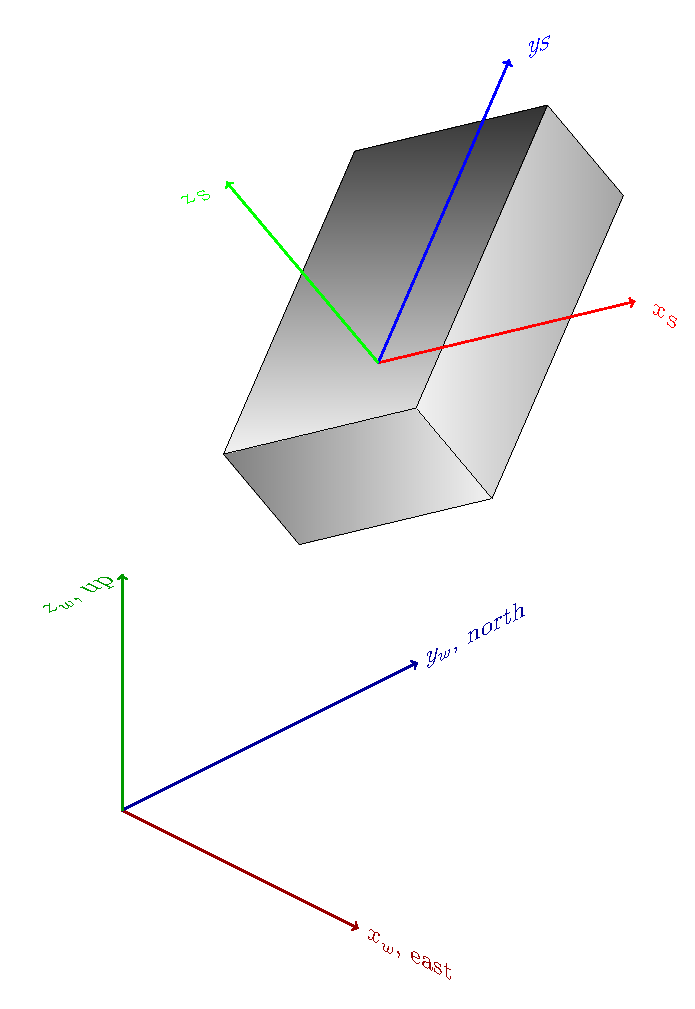
\includegraphics[width=.92\linewidth]{imu-cube}
\end{center}
\end{column}
\begin{column}{0.6\textwidth}
Find the orientation of the IMU (cell phone in our case) with respect to the world fixed frame!
\[ v^W = Rv^S, \qquad v^S = R^T v^W\]
\end{column}
\end{columns}
\end{frame}
\section{EKF}
\label{sec-2}
\begin{frame}[label=sec-2-1]{The Kalman Filter}
\begin{align*}
x_{k+1} &= Fx_k + Bu_k + v_k\\
y_k &= Hx_k+ e_k
\end{align*}
The (filtering) KF provides the pdf $p(x_k|y_{1:k})$. Linear model and Gaussian noise leads to gaussian pdf, completely specified by mean $\hat{x}_{k|k}$ and error covariance $P_{k|k}$. 
\begin{center}
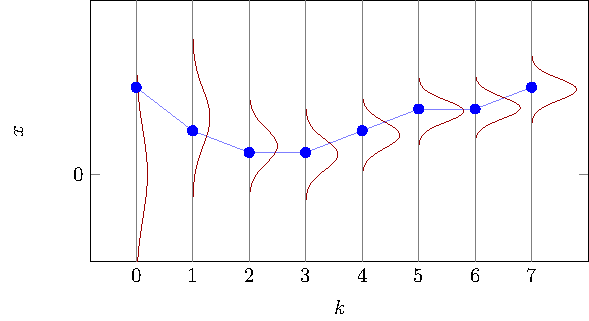
\includegraphics[width=0.6\linewidth]{kf-propagation.pdf}
\end{center}
\end{frame}
\begin{frame}[label=sec-2-2]{The KF algorithm}
Prediction step / time update
\begin{align*} 
\hat{x}_{k+1|k} &= F\hat{x}_{k|k} + Bu_k \quad \text{\textcolor{gray}{predicted state estimate}}\\
P_{k+1|k} &= FP_{k|k}F^T + Q_k \quad \text{\textcolor{gray}{predicted error covariance}}
\end{align*}
Measurement update
\begin{align*}
\tilde{y}_k &= y_k - H\hat{x}_{k|k-1} \quad \text{\textcolor{gray}{innovation}}\\
S_k &= HP_{k|k-1}H^T + R_k \quad \text{\textcolor{gray}{innovation covariance}}\\
K_k &= P_{k|k-1}H^TS_k^{-1}\quad \text{\textcolor{gray}{the Kalman gain}}\\
x_{k|k} &= x_{k|k-1} + K_k\tilde{y}_k \quad \text{\textcolor{gray}{updated state estimate}}\\
P_{k|k} &= (I - K_kH)P_{k|k-1} \quad \text{\textcolor{gray}{Updated error covariance}}
\end{align*}
\end{frame}
\begin{frame}[label=sec-2-3]{The Extended Kalman Filter}
Useful for \emph{nonlinear} state-space models
\begin{align*}
x_{k+1} &= f(x_k, u_k) + v(k)\\
y_k &= h(x_k) + e(k)
\end{align*}
The (filtering) KF provides an \emph{approximation} of the pdf $p(x_k|y_{1:k})$.
\end{frame}
\begin{frame}[label=sec-2-4]{The EKF algorithm}
Prediction step / time update
\begin{align*} 
F_k &= \frac{\partial}{\partial x}f(x,u)|_{x=x_k, u=u_k}\qquad  
B_k = \frac{\partial}{\partial u}f(x,u)|_{x=x_k, u=u_k}\\
\hat{x}_{k+1|k} &= f(\hat{x}_{k|k}, u_k) \quad \text{\textcolor{gray}{predicted state estimate, using nonlinear model}}\\
P_{k+1|k} &= F_kP_{k|k}F_k^T + Q_k \quad \text{\textcolor{gray}{predicted error covariance}}
\end{align*}
Measurement update
\begin{align*}
H_k &= \frac{\partial}{\partial x}h(x)|_{x=x_k}\\
\tilde{y}_k &= y_k - h(\hat{x}_{k|k-1}) \quad \text{\textcolor{gray}{innovation, using nonlinear model}}\\
S_k &= H_kP_{k|k-1}H_k^T + R_k \quad \text{\textcolor{gray}{innovation covariance}}\\
K_k &= P_{k|k-1}H_k^TS_k^{-1}\quad \text{\textcolor{gray}{the Kalman gain}}\\
x_{k|k} &= x_{k|k-1} + K_k\tilde{y}_k \quad \text{\textcolor{gray}{updated state estimate}}\\
P_{k|k} &= (I - K_kH_k)P_{k|k-1} \quad \text{\textcolor{gray}{Updated error covariance}}
\end{align*}
\end{frame}
\section{Quaternions}
\label{sec-3}
\begin{frame}[label=sec-3-1]{Describing orientations using unit quaternions}
The unit quaternion $q= \begin{bmatrix}q_0& q_1 & q_2 & q_3 \end{bmatrix}^T$, can represent a 3D rotation of angle $\alpha$ about the direction $v=\begin{bmatrix}v_x & v_y & v_z\end{bmatrix}^T$
\begin{equation*}
q = \begin{bmatrix}q_0\\ q_1 \\ q_2 \\ q_3 \end{bmatrix}
  = \begin{bmatrix} \cos(\frac{1}{2}\alpha)\\ \sin(\frac{1}{2}\alpha) \begin{bmatrix} v_x\\v_y\\v_z\end{bmatrix} \end{bmatrix} = \begin{bmatrix} \cos(\frac{1}{2}\alpha)\\\sin(\frac{1}{2}\alpha) v \end{bmatrix}
\end{equation*}
\end{frame}
\begin{frame}[label=sec-3-2]{From quaternion to rotation matrix}
There are straight-forward formulas to convert a unit quaternion to a rotation matrix and vice versa
\[R = Q(q), \qquad q = Q^{-1}(R),\]
where 
\[Q(q) = \begin{bmatrix} 2q_0^2-1+2q_1^2 & 2q_1q_2-2q_0q_3 & 2q_1q_3 + 2q_0q_2\\
   2q_1q_2 + 2q_0q_3 & 2q_0^2-1+2q_2^2 &2q_2q_3-2q0q_1\\
   2q_1q_3-2q_0q_2 & 2q_2q_3+2q_0q_1 &2q_0^2-1+2q_3^2 \end{bmatrix} \]
\end{frame}
\begin{frame}[label=sec-3-3]{The time-derivative of a unit quaternion}
\[ \dot{q} = \frac{1}{2}S(\omega) q, \quad \text{where} \]
\[ S(\omega) = \begin{bmatrix} 0 & -\omega_x & -\omega_y & -\omega_z\\
   \omega_x & 0 & \omega_z & -\omega_y\\
   \omega_y & -\omega_z & 0 & \omega_x\\
   \omega_z & \omega_y & -\omega_x & 0 \end{bmatrix} \]
\end{frame}

\begin{frame}[label=sec-3-4]{The state-vector}
There are a two main alternatives 
\begin{enumerate}
\item \[ x_k = q_k\]
\item \[ x_k = \begin{bmatrix} q_k\\ w_k\end{bmatrix}, \]
      where \(w_k\) is the gyro bias.
\end{enumerate}
\end{frame}

\begin{frame}[label=sec-3-5]{Integrating angular velocities}
The orientation quaternion can be updated from gyro measurements, $\omega_k$
\begin{align*}
 q_{k+1} &= \mathrm{e}^{\frac{1}{2}S(\omega_k)h} q_k\\
 \underbrace{q_{k+1}}_{x_{k+1}} &= \underbrace{\left( \cos(\frac{||\omega_k||h}{2})I + \frac{h}{2}\cdot\frac{\sin(\frac{||\omega_k||h}{2})}{\frac{||\omega_k||h}{2}}S(\omega_k)\right)}_{F_k} \underbrace{q_k}_{x_k} + v_k,
 \end{align*}
where $h$ is the sampling period (which need not be constant). 
\end{frame}

\section{IMU measurements}
\label{sec-4}
\begin{frame}[label=sec-4-1]{The accelerometer measurement}
The accelerometer measures both the gravitational acceleration $g^0$ and the acceleration of the IMU itself wrt the earth, $a^f_k$, called the \emph{specific force}.
\[ y_k^a = R^T(g^0 + a_k^f) + e_k^a = Q^T(q_k)\big(g^0 + a_k^f\big) + e_k^a\]
Assuming negligable specific force, $a_k^f\approx 0$:
\[ y_k^a = \underbrace{Q^T(q_k)g^0}_{h_a(x)} + e_k^a\]
For the EKF we need the derivative of $h^a(x)$ wrt $x$
\[ H^a_k = \frac{\partial}{\partial x}h^a(x)|_{x_k} = \begin{bmatrix}H^a_{k,0} & H^a_{k,1} & H^a_{k,2} & H^a_{k,3}\end{bmatrix}, \]
where
\[H^a_{k,0} = \left(\frac{\partial}{\partial q_0}Q^T(q)\right)\Big|_{q_k}g^0, \; H^a_{k,1} = \left(\frac{\partial}{\partial q_1}Q^T(q)\right)\Big|_{q_k}g^0, \; \text{etc.}\]
\end{frame}

\begin{frame}[label=sec-4-2]{The magnetometer measurement}
The magnetometer measures the local magnetic field (hopefully dominated by the earth's magnetic field)
\[ y_k^m = R^T(m^0) + e_k^m = \underbrace{Q^T(q)m^0}_{h^m(x)} + e_k^m\]
\[ H^m_k = \frac{\partial}{\partial x}h^m(x)|_{x_k} = \begin{bmatrix}H^m_{k,0} & H^m_{k,1} & H^m_{k,2} & H^m_{k,3}\end{bmatrix}, \]
where
\[H^m_{k,0} = \left(\frac{\partial}{\partial q_0}Q^T(q)\right)\Big|_{q_k}m^0, \; H^m_{k,1} = \left(\frac{\partial}{\partial q_1}Q^T(q)\right)\Big|_{q_k}m^0, \; \text{etc.}\]
\end{frame}

\section{Hands-on}
\label{sec-5}
\begin{frame}[label=sec-5-1]{Hands-on}
\begin{block}{Set-up Wireless IMU}
\end{block}
\begin{block}{Plot some data}
\end{block}
\begin{block}{Implement time update}
\end{block}
\begin{block}{Implement measurement updates}
\end{block}
\end{frame}
% Emacs 25.3.50.2 (Org mode 8.2.10)
\end{document}